\documentclass[10pt]{article}

\PassOptionsToPackage{hidelinks}{hyperref}
\usepackage[utf8]{inputenc}
\usepackage{amsmath, calc, xcolor}
\usepackage{alphabeta} 
\usepackage[pdftex]{graphicx}
\usepackage[top=1in, bottom=1in, left=1in, right=1in]{geometry}
\usepackage[]{bookmark}
\linespread{1.06}
\setlength{\parskip}{8pt plus2pt minus2pt}

\widowpenalty 10000
\clubpenalty 10000

\newcommand{\eat}[1]{}
\newcommand{\HRule}{\rule{\linewidth}{0.5mm}}
\usepackage[official]{eurosym}
\usepackage{enumitem}
\setlist{nolistsep,noitemsep}
\usepackage[]{hyperref}
\usepackage{url}
\usepackage{cite}
\usepackage{lipsum}
\usepackage{indentfirst}
\usepackage{tikz}
\usetikzlibrary{arrows,decorations.pathmorphing,backgrounds,fit,positioning,shapes.symbols,chains}
\usepackage{xcolor,colortbl}
\usepackage{array}

\setlength{\parindent}{2em}
\renewcommand*\contentsname{Índice}
\renewcommand\refname{}

\begin{document}

%===========================================================
\begin{titlepage}
\begin{center}

% Top 

\includegraphics[width=0.55\textwidth]{img/logo-isec-transparente.png}~\\[2cm]


% Title
\HRule \\[0.4cm]
{ \LARGE 
  \textbf{Inteligência Computacional}\\[0.4cm]
}
\HRule \\[1.5cm]

% Docente
{ \large
  \textbf{Docente} \\[0.1cm]
  Inês Dominguês \\ Carlos Pereira \\[2.5cm]
}


% Author
{ \large
  \textbf{Alunos} \\[0.1cm]
  Paulo Henrique Figueira Pestana de Gouveia - a2020121705 \\[0.1cm]
  Nuno Alexandre Almeida Santos - a2019110035\\[0.1cm]
}

\vfill



% Bottom
{\large \today}
 
\end{center}
\end{titlepage}


\newpage



%===========================================================
\tableofcontents
\addtocontents{toc}{\protect\thispagestyle{empty}}
\newpage
\setcounter{page}{1}

%===========================================================
%===========================================================
\large
\section{Introdução}\label{sec:intro}

\section{Em que consiste a Computação Evolucionária?}\label{sec:comp-evo}
    A evolução é um processo de otimização em que o objetivo é melhorar a capacidade de um organismo (ou sistema) sobreviver em ambientes dinâmicos e competitivos.
    Ao falar sobre evolução, é importante primeiro identificar a área em que a evolução pode ser definida, por exemplo, cósmica, química, estelar e planetária,
sistemas de evolução orgânicos ou feitos pelo homem. Para essas diferentes áreas, a evolução pode
ser interpretado de forma diferente. 
    A Computação Evolucionária compreende um conjunto de técnicas de busca e otimização inspiradas na 
evolução natural das espécies. Desta forma, cria-se uma população de indivíduos que vão reproduzir e 
competir pela sobrevivência. Os melhores sobrevivem e transferem suas características a novas gerações.


\subsection{Descrição do paradigma de computação evolucionária e possíveis aplicações no contexto de treino de uma rede neuronal}\label{sec:apre-da-org}

\section{Inteligência Swarm}\label{sec:ev-da-org}
Conjunto estruturado de indivíduos (ou agentes) que interagem entre si.
Os Indivíduos pertencentes ao swarm (enxame) interagem para atingirem um objectivo comum,
de forma mais eficiente do que agindo individualmente.
Formalmente, um enxame pode ser definido como um grupo de agentes (geralmente móveis) que se comunicam entre si (seja direta ou indiretamente), agindo no seu ambiente local.
 Mais formalmente, inteligência Swarm é a propriedade de um sistema pelo qual os comportamentos coletivos de agentes não sofisticados interagindo localmente com seu ambiente causam o surgimento de padrões funcionais globais coerentes.
 O objetivo dos modelos computacionais de inteligência Swarm é modelar o simples
comportamento dos indivíduos e as interações locais com o ambiente e os indivíduos vizinhos, a fim de obter comportamentos mais complexos que podem ser usados para resolver problemas complexos, principalmente problemas de otimização.

Inteligência Swarm faz uso de algoritmos de convergência baseados em fenômenos emergentes da natureza como: colônias de insetos, estratégias coletivas de peixes e pássaros e ainda comportamento auto-organizativo de partículas atômicas e subatômicas.

Por outro lado, a otimização de colônia de formigas modela o comportamento muito simples de seguir a trilha de feromônio das formigas, onde cada formiga percebe as concentrações de feromônio em sua
ambiente local e age selecionando probabilisticamente a direção com maior
concentração de feromônio. Daí surge o comportamento de encontrar a melhor alternativa (caminho mais curto) a partir de uma coleção de alternativas. Modelos do comportamento local de
formigas que frequentam cemitérios resultam no comportamento complexo de agrupar objetos semelhantes
em clusters.

\subsection{PSO}\label{sec:PSO}
O algoritmo de otimização de enxame de partículas (PSO) é um algoritmo de pesquisa baseado em população baseado na simulação do comportamento social de pássaros dentro de um bando, que são denominados por partículas. Esse método se inicializa aleatoriamente, através de um conjunto de partículas com velocidades e posições aleatórias. Após essa inicialização os indivíduos são avaliados através da função de avaliação. Em um algoritmo PSO existe um conjunto de vetores cujas trajetórias oscilam em torno de uma região definida por cada melhor posição individual (PBEST) e a melhor posição dos outros (GBEST).

A posição da partícula, xi, vai sendo atualizada de acordo com a equação:
\begin{equation}
  \vspace{1cm}
    xi (t+1) = xi (t) + w.vi(t) + C1.rnd(PBEST ‐ xi (t)) + C2.rnd(GBEST ‐ xi (t))
\end{equation}
Na equação (1), vi(t) representa o vetor velocidade da partícula i no tempo t, w é o fator de inércia, rnd representa números aleatórios de distribuição uniforme entre 0‐1, C1 e C2 representam respectivamente os parâmetros social e cognitivo, PBEST é a melhor posição individual e GBEST é a melhor posição social. Os parâmetros C1 e C2 ajustam o balanço entre a influência social e a aprendizagem da partícula individual.

Algoritmo de otimização de enxame de partículas (PSO) modela dois comportamentos simples:  cada indivíduo (1) se move em direção seu melhor vizinho mais próximo e  (2) retorna ao estado que o indivíduo experimentou ser o melhor para si mesmo. Como resultado, o comportamento coletivo que emerge é que
de todos os indivíduos convergindo para o estado ambiental que é melhor para todos os indivíduos.

Exempo:

Uma forma mais simples de explicação pode ser um bando de gaivotas telepáticas à procura da melhor fonte de comida. Todas começam num mapa distribuídas aleatoriamente, no inicio antes de se moverem têm velocidade
zero mas sabem qual a gaivota mais próximo da solução ótima, alteram então a sua velocidade e direcção para
irem nesse sentido. À medida que vão andando vão-se lembrando da sua melhor posição, usam a sua velocidade actual, a sua melhor posição e a melhor posição global para alterarem a sua velocidade e logo a sua
posição para se dirigirem para a posição óptima. Como iniciaram em posições aleatórias no mapa ao dirigirem-se todas para o mesmo ponto inevitavelmente vão passar pelo ponto óptimo, alterando ao
melhor global e fazendo com que todas consigam convergir nesse ponto.

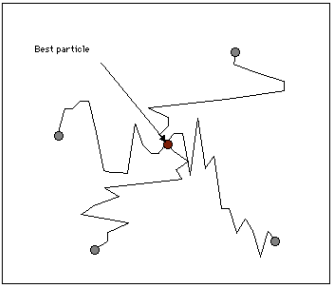
\includegraphics{img/PSO.png}

\section{FireFly}\label{sec:firefly}
A maioria das espécies de vaga-lumes são capazes de brilhar produzindo flashes curtos. Considera-se que a principal função 
dos flashes é atrair vaga-lumes do sexo oposto e potenciais presas. Além disso, um flash de sinal pode comunicar a um 
predador que um vaga-lume tem um gosto amargo. 

  \section{Particle Swarm Otimization. Quais as vantagens e desvantagens?}\label{sec:sworm}
  O Algoritmo Firefly é baseado em duas coisas importantes: a mudança na intensidade da luz e atratividade. Para simplificar, 
  assume-se que a atratividade de um vaga-lume é definida por seu brilho que está relacionado com a função objetivo.
  O algoritmo utiliza o seguinte modelo de comportamento do vaga-lume: 
\begin{enumerate}
  \item Todos os vaga-lumes são capazes de se atrair independentemente do sexo; 
  \item A atratividade de um vaga-lume para outros indivíduos é proporcional ao seu brilho. 
  \item Vaga-lumes menos atraentes se movem na direção do mais atraente. 
  \item À medida que a distância entre dois vaga-lumes aumenta, o brilho visível de um determinado vaga-lume para o outro diminui. 
  \item Se um vaga-lume não vê nenhum vaga-lume que seja mais brilhante do que ele, ele se move aleatoriamente. 
\end{enumerate}

\subsection{Descrever em detalhe o algoritmo selecionado e apresentar uma análise comparativamente com a versão base, o PSO.}\label{sec:desc-algo}

\section{Análsie de desempenho}\label{sec:an-desem}
\subsection{Aplicar e ilustrar ao algoritmo para otimização de duas funções “benchmark” a função esfera (para dimensão 2 e 3) e função de Ackley (para dimensão 2 e 3).}\label{sec:apre-da-org}
\subsection{Comparar com a versão base do PSO e analisar a sensibilidade aos diferentes parâmetros do algoritmo, apresentando tabela com resultados.}\label{sec:apre-da-org}

\section{Conclusões}\label{sec:conc}

\vspace{1cm}

\section{Referências}\label{sec:sup-inf-utl}
\bibliographystyle{ieeetr}
\bibliography{refs}


%===========================================================

%===========================================================

\pagebreak
\end{document} 
